\documentclass[a4paper,10pt]{jsarticle}

% 数式
\usepackage{amsmath,amsfonts}
\usepackage{bm}
% 画像
\usepackage[dvipdfmx]{graphicx}
\usepackage{here}

\usepackage{url}

\usepackage{listingsutf8,jlisting} %日本語のコメントアウトをする場合jlistingが必要
%ここからソースコードの表示に関する設定
\lstset{
  basicstyle={\ttfamily},
  identifierstyle={\small},
  commentstyle={\smallitshape},
  keywordstyle={\small\bfseries},
  ndkeywordstyle={\small},
  stringstyle={\small\ttfamily},
  frame={tb},
  breaklines=true,
  columns=[l]{fullflexible},
  numbers=left,
  xrightmargin=0zw,
  xleftmargin=3zw,
  numberstyle={\scriptsize},
  stepnumber=1,
  numbersep=1zw,
  lineskip=-0.5ex
}

\begin{document}

\title{オペレーティングシステム演習4}
\author{坪井正太郎(101830245)}
\date{\today}
\maketitle

\section{問題1}
\subsection{メモリ配置図}
\begin{figure}[H]
  \begin{tabular}{cc}
    %---- 最初の図 ---------------------------
    \begin{minipage}[t]{0.45\hsize}
      \centering
      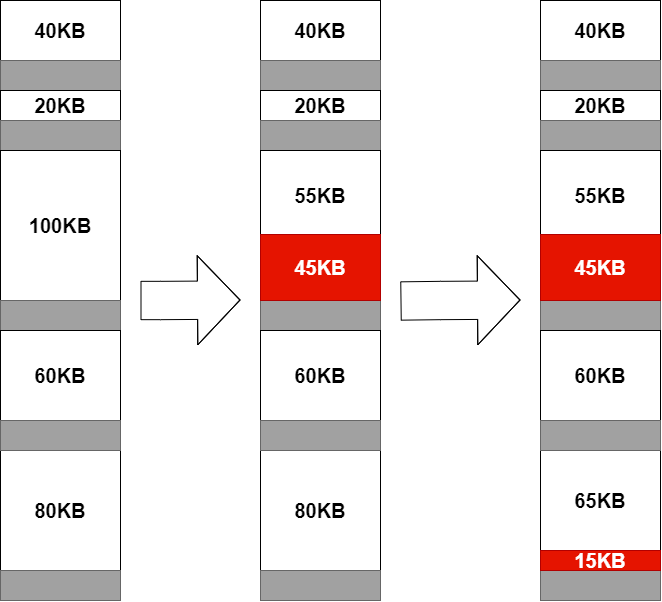
\includegraphics[width=6cm]{./01.drawio.png}
      \caption{worst-fit}
      \label{worst-fit}
    \end{minipage} &
    %---- 2番目の図 --------------------------
    \begin{minipage}[t]{0.45\hsize}
      \centering
      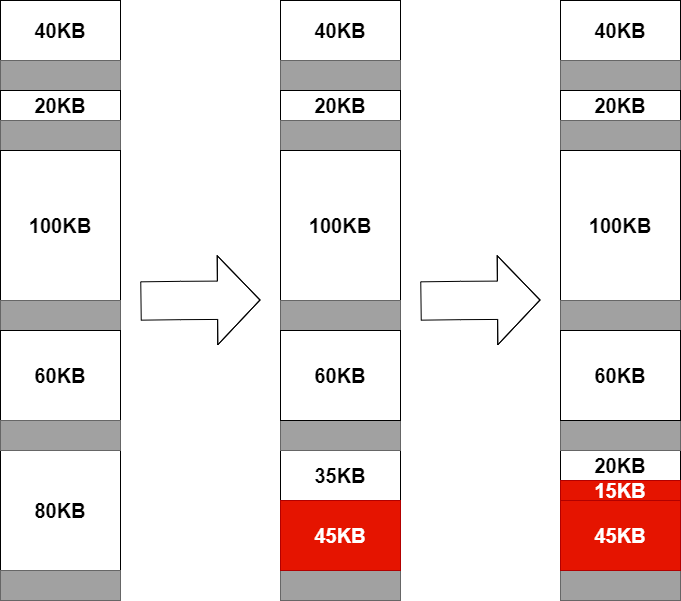
\includegraphics[width=6cm]{./02.drawio.png}
      \caption{first-fit}
      \label{first-fit}
    \end{minipage}
    %---- 図はここまで ----------------------
  \end{tabular}
\end{figure}

\begin{figure}[H]
  \centering
  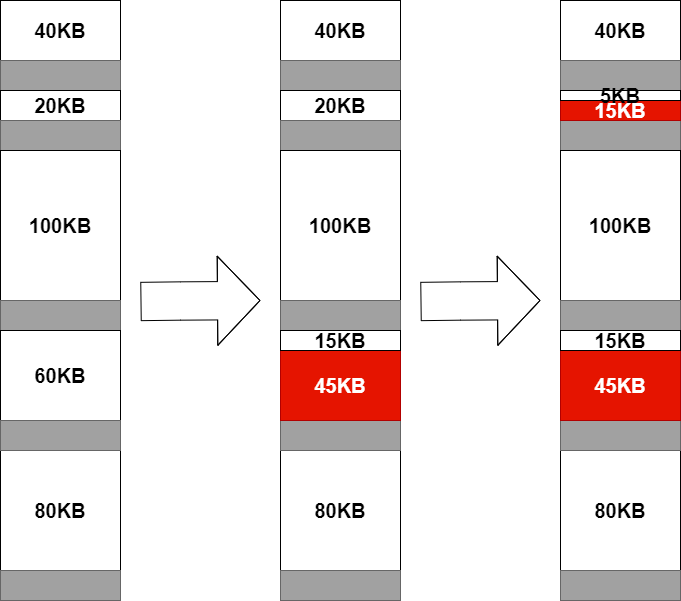
\includegraphics[width=6cm]{./03.drawio.png}
  \caption{best-fit}
  \label{best-fit}
\end{figure}

\newpage
\subsection{50\%ルールの導出}
$N$をプロセスの総数、$M$を空き領域の総数とする。
プロセスのうち、両隣とも空き領域のものを$N_A$、片隣のみ空き領域のものを$N_B$、両隣とも空き領域でないものを$N_C$とする。

このとき、\[N=N_A+N_B+N_C\] \[M=\frac{2N_A+N_B}{2}\]が成り立つ。
定常状態のとき、$M$の増加数と減少数は等しくなる。
プロセスが生成される確率を$P_s$開放される確率を$P_e$とすると、$M$の増加数は$P_e\left(\frac{N_C}{N}\right)$減少数は\(P_e\left(\frac{N_A}{N}\right)\)となり、定常状態のとき次の等式が成り立つ。
\[P_e\left(\frac{N_C}{N}\right)=P_e\left(\frac{N_A}{N}\right)\]
\[N_C=N_A\]
よって、
\[N=N_A+N_B+N_C=2N_A+N_B\]となり、\(M=\frac{N}{2}\)となるので空き領域の個数は使用中領域のおよそ半分になる。

\section{問題2}
\subsection{K\&R malloc}
K\&Rのmalloc.cでは、未使用領域のヘッダをつなげた連結リストを探索することによる、first-fitでメモリ領域の割付を行っている。
また、freeは空き領域サイズの更新とポインタの付替えで実装している。

空き領域も確保された領域も、HAEDER構造体が領域の先頭についている。
(HEADERは、領域のサイズと次の空き領域へのポインタをもつ)
このうち、空き領域の部分のみをアドレス順に連結リストとしてつないでいる。
\subsubsection{malloc}
mallocの際は確保に十分な空き領域のサイズを、確保したいサイズ+HEADER分縮めることでその領域を確保する。
空き領域が確保したいサイズよりも大きい場合には空き領域の連結リストを更新する必要はないが、空き領域と確保したい領域サイズが等しい場合、ひとつ前の空き領域からのポインタを次のポインタに移し替えることでリストに空き領域しか入らないようにしている。

また、freeでの探索と、mallocで確保する領域の探索のために、最後に操作された空き領域はグローバル変数として記憶される。
これは、確保されたメモリは近いうちに開放されることが多いという特性を利用する目的と、リストの先頭側ばかりが確保され、フラグメンテーションが進むことを回避する目的のためである。

空き領域が足りない場合は、ヒープ領域を伸ばすbrkシステムコールを使用して新たに領域を確保する。

\subsubsection{free}
freeでは前後の空き領域と結合、ポインタ差し替えを行うために、現在の空き領域を探索し、予め前後の空き領域を持っておく。
このとき、mallocで記憶された領域位置から線形リストの探索が行われる。

領域を空き領域にする際、次の空き領域が右に隣接しているかいないか、前の空き領域が左に隣接しているかいないかの判定を行い、空き領域リストに過不足がないようにサイズと次の領域を指すポインタを変更している。

\subsection{glibc malloc}
glibcのmalloc実装では、HEADERのメンバを増やし、前の領域のサイズと前後のポインタを持っておくことで、freeでの空き領域結合の効率を上げている。
また、空き領域を管理するためのリストを容量ごとに用意することで、best-fitでのmallocを高速に行うことができる。

\subsubsection{malloc}
mallocでは、確保したい領域のサイズに合うようなリストを探索してそのサイズに合った領域を割り当てる。
また、新たに追加したHEADERメンバのうち、確保済みの領域については必要のないメンバがあり、その部分を差し引いてユーザーに渡すことでヒープ領域の空間効率を向上させている。

\subsubsection{free}
free時に、削減されていたメンバを書き込み、前後の空き領域と結合する。
また、即座に空き領域同士を結合せず、サイズをそのままにしておくことで同じサイズの構造体が連続してmalloc-freeされた際の性能を上げている。

\subsection{比較}
K\&R実装はコードサイズが小さく、十分に大きい空き領域が存在する場合にはmallocのオーバーヘッドが少ない。
しかし、first-fitによる割付では、確保されたサイズによってはフラグメンテーションが進んでしまい、brkが呼ばれてしまう。
brkはmalloc.cによる処理よりも大幅に遅いので、不利に働く。

一方、glibcのmalloc実装は、サイズごとに空き領域リストを管理しており、メモリのフラグメンテーションが起こりにくい。
また、free時にリストを巡回する必要がないので、結合操作をより高速にできるという利点がある。
ヘッダサイズの増加による空間効率の悪化も、ユーザーに渡す際には上書き可能となるため、実質的なデメリットにはなっていないと考えられる。

したがって、実装の重さを除けばほとんどの場合においてglibc実装の方が効率、速度ともに有利であると言える。

\end{document}
